\documentclass[10pt]{article}
\usepackage[pdftex]{graphicx}
\usepackage[utf8]{inputenc}
\usepackage{amsmath}
\usepackage{enumerate}
\usepackage{alltt}
\usepackage{float}
\usepackage{bbold}
\usepackage{caption}
\usepackage{subcaption}
\usepackage{subfig}
\restylefloat{table}
\usepackage{appendix}

\title{Symbolic Execution in Ruby\\
CMSC 631 Final Project}
\author{Elizabeth McNany and David Wasser}
\date{May 16, 2013}

\begin{document}
\maketitle

\begin{abstract}
Here is an abstract
\end{abstract}

\section{Introduction}
Motivation stuff goes here \cite{typeinf} \cite{rails}

\section{Methodology}
methodology junk goes here

\subsection{Proxies}
We use proxies as a wrapper around objects to bundle the actual value and symbolic variable during execution.  Typically, a variable name points to its value in working memory as shown in Figure \ref{pointer:1}.  We add an additional layer with the proxy wrapper, as in Figure \ref{pointer:2}.  The program accesses only the proxy directly, which contains a reference to the variable, which then points to the actual value.

\begin{figure}
  \centering
  \begin{subfigure}{0.5\textwidth}
	\centering
	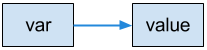
\includegraphics[height=25px]{pointer1.png}
	\caption{Variable in original program.}
	\label{pointer:1}
  \end{subfigure}\begin{subfigure}{0.5\textwidth}
	\centering
	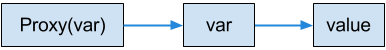
\includegraphics[height=25px]{pointer2.png}
	\caption{Proxied variable representation.}
	\label{pointer:2}
  \end{subfigure}
  \caption{Representation of a normal vs. proxied variable.}
\end{figure}

This is accomplished via Ruby's built-in \texttt{coerce} and \texttt{method\_missing} classes.  These methods are part of the Ruby language and implementation and are called on a variable if it does not have particular properties.  By overriding these functions, we can catch method calls using the proxied variable and store the variable information, argument, and function at the time of call to pass on to the SMT solver.\\

Specifically, \texttt{method\_missing} is called on the object if the object does not have a particular method defined, passing in the information for the original function call.  The default behavior of the Ruby interpreter is to simply raise an exception.\\

When an object that has been passed as an argument to another method which requires a specific type, but the object does not have a defined conversion to that type, the \texttt{coerce} method is called on that object.  If no suitable conversion is found, an exception will be raised.\\

\subsection{Z3}
stuff about z3

\section{Implementation}
There are two main components of our implementation: the Z3 API and the proxy class for variables.

We have implemented proxy classes for both Ruby Fixnums and Booleans.

\section{Assessment}
using short ruby programs, see appendix

\section{Conclusion}
Summary and Future Work
More types of variables

\begin{thebibliography}{99}
\bibitem{rails}
A. Chaudhuri and J. Foster, ``Symbolic Security Analysis of Ruby-on-Rails Web Applications,'' in Proceedings of the 17th ACM Conference on Computer and Comm. Security, 2010, pp. 585-594.

\bibitem{typeinf}
B. Ren, J. Toman, T. S. Strickland, J. Foster, ``The Ruby Type Checker,'' in SAC '13: Proceedings of the 28th Annual ACM Symposium on Applied Computing, 2013.

\end{thebibliography}

\appendix
\section{Program 1}
\begin{verbatim}
Code goes here
\end{verbatim}

\end{document}
